%-----------------------------------------------------------------------------------------------------------------------------------------------%
%	The MIT License (MIT)
%
%	Copyright (c) 2022 Gauthier Cart
%
%	Permission is hereby granted, free of charge, to any person obtaining a copy
%	of this software and associated documentation files (the "Software"), to deal
%	in the Software without restriction, including without limitation the rights
%	to use, copy, modify, merge, publish, distribute, sublicense, and/or sell
%	copies of the Software, and to permit persons to whom the Software is
%	furnished to do so, subject to the following conditions:
%
%	THE SOFTWARE IS PROVIDED "AS IS", WITHOUT WARRANTY OF ANY KIND, EXPRESS OR
%	IMPLIED, INCLUDING BUT NOT LIMITED TO THE WARRANTIES OF MERCHANTABILITY,
%	FITNESS FOR A PARTICULAR PURPOSE AND NONINFRINGEMENT. IN NO EVENT SHALL THE
%	AUTHORS OR COPYRIGHT HOLDERS BE LIABLE FOR ANY CLAIM, DAMAGES OR OTHER
%	LIABILITY, WHETHER IN AN ACTION OF CONTRACT, TORT OR OTHERWISE, ARISING FROM,
%	OUT OF OR IN CONNECTION WITH THE SOFTWARE OR THE USE OR OTHER DEALINGS IN
%	THE SOFTWARE.
%-----------------------------------------------------------------------------------------------------------------------------------------------%

%----------------------------------------------------------------------------------------
%   DOCUMENT
%----------------------------------------------------------------------------------------
\documentclass[10pt,A4]{article}
\usepackage[utf8]{inputenc}
\usepackage{xifthen}

%----------------------------------------------------------------------------------------
%   PAGE LAYOUT
%----------------------------------------------------------------------------------------
\usepackage[a4paper]{geometry}
\usepackage{fancyhdr}

\geometry{top=1.75cm, bottom=-.6cm, left=1.5cm, right=1.5cm}
\pagestyle{fancy}
\setlength{\headheight}{-5pt}
\setlength{\parindent}{0mm}

%----------------------------------------------------------------------------------------
%   FONTS
%----------------------------------------------------------------------------------------
\usepackage[default]{raleway}
\usepackage[T1]{fontenc}
\usepackage{fontawesome5}
\usepackage{worldflags}
\usepackage[hidelinks,unicode]{hyperref}
\usepackage{moresize}
\renewcommand*\familydefault{\sfdefault}
\newcommand*{\fontdir}[1][fonts/]{\def\@fontdir{#1}}
\fontdir

\newfontfamily\monoregular[
    Path=\@fontdir,
    UprightFont=*-Regular,
    ItalicFont=*-RegularItalic,
    BoldFont=*-Bold,
    BoldItalicFont=*-BoldItalic,
]{MonoLisa}

\newfontfamily\monolight[
    Path=\@fontdir,
    UprightFont=*-Light,
    ItalicFont=*-LightItalic,
    BoldFont=*-Medium,
    BoldItalicFont=*-MediumItalic,
]{MonoLisa}

\newfontfamily\helveticamedium[
    Path=\@fontdir,
    UprightFont=*-Medium,
    ItalicFont=*-MediumItalic,
    BoldFont=*-Bold,
    BoldItalicFont=*-BoldItalic,
]{HelveticaNeue}

\newfontfamily\helveticalight[
    Path=\@fontdir,
    UprightFont=*-Light,
    ItalicFont=*-LightItalic,
    BoldFont=*-Medium,
    BoldItalicFont=*-MediumItalic,
]{HelveticaNeue}

%----------------------------------------------------------------------------------------
%   ARRAY DEFINITION
%----------------------------------------------------------------------------------------

\usepackage{multicol}
\usepackage{multirow}
\usepackage{array}

\newcolumntype{x}[1]{%
        >{\raggedleft\hspace{0pt}}p{#1}}%

%----------------------------------------------------------------------------------------
%   GRAPHICS DEFINITION
%----------------------------------------------------------------------------------------

\usepackage{graphicx}
\usepackage{wrapfig}
\usepackage{float}
\usepackage{tikz}
\usetikzlibrary{shapes, backgrounds,mindmap, trees}

%----------------------------------------------------------------------------------------
%   COLOR DEFINITION
%----------------------------------------------------------------------------------------
\usepackage{color}

\definecolor{black}{HTML}{000000}
\definecolor{purple}{HTML}{635Bff}
\definecolor{indigo}{HTML}{0A2540}
\definecolor{lightblue}{HTML}{00D4FF}
\definecolor{gray}{HTML}{BEBEBE}

%----------------------------------------------------------------------------------------
%   HEADER
%----------------------------------------------------------------------------------------
\renewcommand{\headrulewidth}{0pt}
\renewcommand{\footrulewidth}{0pt}
\renewcommand{\thepage}{}
\renewcommand{\thesection}{}

\newcommand{\headicon}[2]
{
    \small
    \hspace{0.1cm}\color{purple}{#1}\hspace{0.1cm}
    \color{black}{#2}
}

\lhead{}
\chead{
        {\headicon
    {\faGraduationCap}
    {Senior Software Engineer}
    }$\cdot$
        {\headicon
    {\faHome}
    {Les Houches, France}
    }$\cdot$
        {\headicon
    {\faPaperPlane}
    {\textcolor{lightblue}{\textbf{gauthier.cart@gmail.com}}}
    }$\cdot$
        {\headicon
    {\faPhone}
    {+33 7 81 64 50 02}
    }
}
\rhead{}

%----------------------------------------------------------------------------------------
%	CV SECTIONS
%----------------------------------------------------------------------------------------

\newcommand{\cvsection}[2]
{
    \vspace{8pt}
    \colorbox{indigo}{\mystrut \makebox[1\linewidth][l]{
        \large\color{lightblue}#1 \hspace{8pt} \textcolor{white}{\textbf{#2}}\hspace{4pt}
    }}\\
}

\newcommand{\metasection}[2]
{
    \begin{tabular*}{1\textwidth}{p{0.5cm} p{2.0cm} p{11cm}}
        \textcolor{purple}{\faAngleDoubleRight}&\normalsize{\textcolor{purple}{#1:}}&#2\\[12pt]
    \end{tabular*}
}

%----------------------------------------------------------------------------------------
%	CV COMPONENTS
%----------------------------------------------------------------------------------------

\newcommand{\cvevent}[5]
{
    \vspace{8pt}
    \begin{tabular*}{1\textwidth}{p{2.3cm}  p{4.8cm} x{9.9cm}}
        \textcolor{black}{#1}& \textbf{#2} & \vspace{2.5pt}\textcolor{lightblue}{#3}

    \end{tabular*}
    \vspace{-12pt}
    \textcolor{gray}{\hrule}
    \vspace{6pt}
    \begin{tabular*}{1\textwidth}{p{2.3cm} p{14.4cm}}
        &\textcolor{purple}{\faAngleDoubleRight}\hspace{4pt}#4\\[3pt]
        &\textcolor{purple}{\faAngleDoubleRight}\hspace{4pt}#5\\[6pt]
    \end{tabular*}

}

\newcommand{\cveventmeta}[2]
{
    \mbox{\mystrut \hspace{87pt}\textit{#1}}\\
    #2
}

\newcommand{\cvflag}[1]
{
    \flagsdefault[width=3mm]
    \vspace{+10pt}\hspace{-6pt}\worldflag{#1}\hspace{-6pt}
}

\newcommand{\cvlink}[2]
{
    \href{#1}{\textcolor{purple}{\hspace{-1pt}#2}}
}

%----------------------------------------------------------------------------------------
%   CUSTOM STRUT FOR EMPTY BOXES
%----------------------------------------- -----------------------------------------------
\newcommand{\mystrut}{\rule[-.3\baselineskip]{0pt}{\baselineskip}}

%============================================================================%
%	DOCUMENT CONTENT
%============================================================================%
\begin{document}

    \pagestyle{fancy}

%---------------------------------------------------------------------------------------
%	TITLE HEADLINE
%----------------------------------------------------------------------------------------
    \vspace{-20.55pt}

    \hspace{-0.25\linewidth}\colorbox{indigo}{
        \makebox[1.5\linewidth][c]{
            \HUGE{
                \textcolor{white}{\textsc{Gauthier Cart}}
                \textcolor{lightblue}{\rule[-1mm]{1mm}{0.9cm}}
                \HUGE{\textcolor{white}{\textsc{34 y/o}} }
            }
        }
    }

%----------------------------------------------------------------------------------------
%	HEADER IMAGE
%----------------------------------------------------------------------------------------

    \begin{figure}[H]
        \begin{flushright}
            \begin{tikzpicture}
                \begin{scope}
                    \clip [rounded corners=2cm] (0,0) rectangle (4cm,4cm);
                    \node[anchor=south west,inner sep=0] (image) at (0,0) {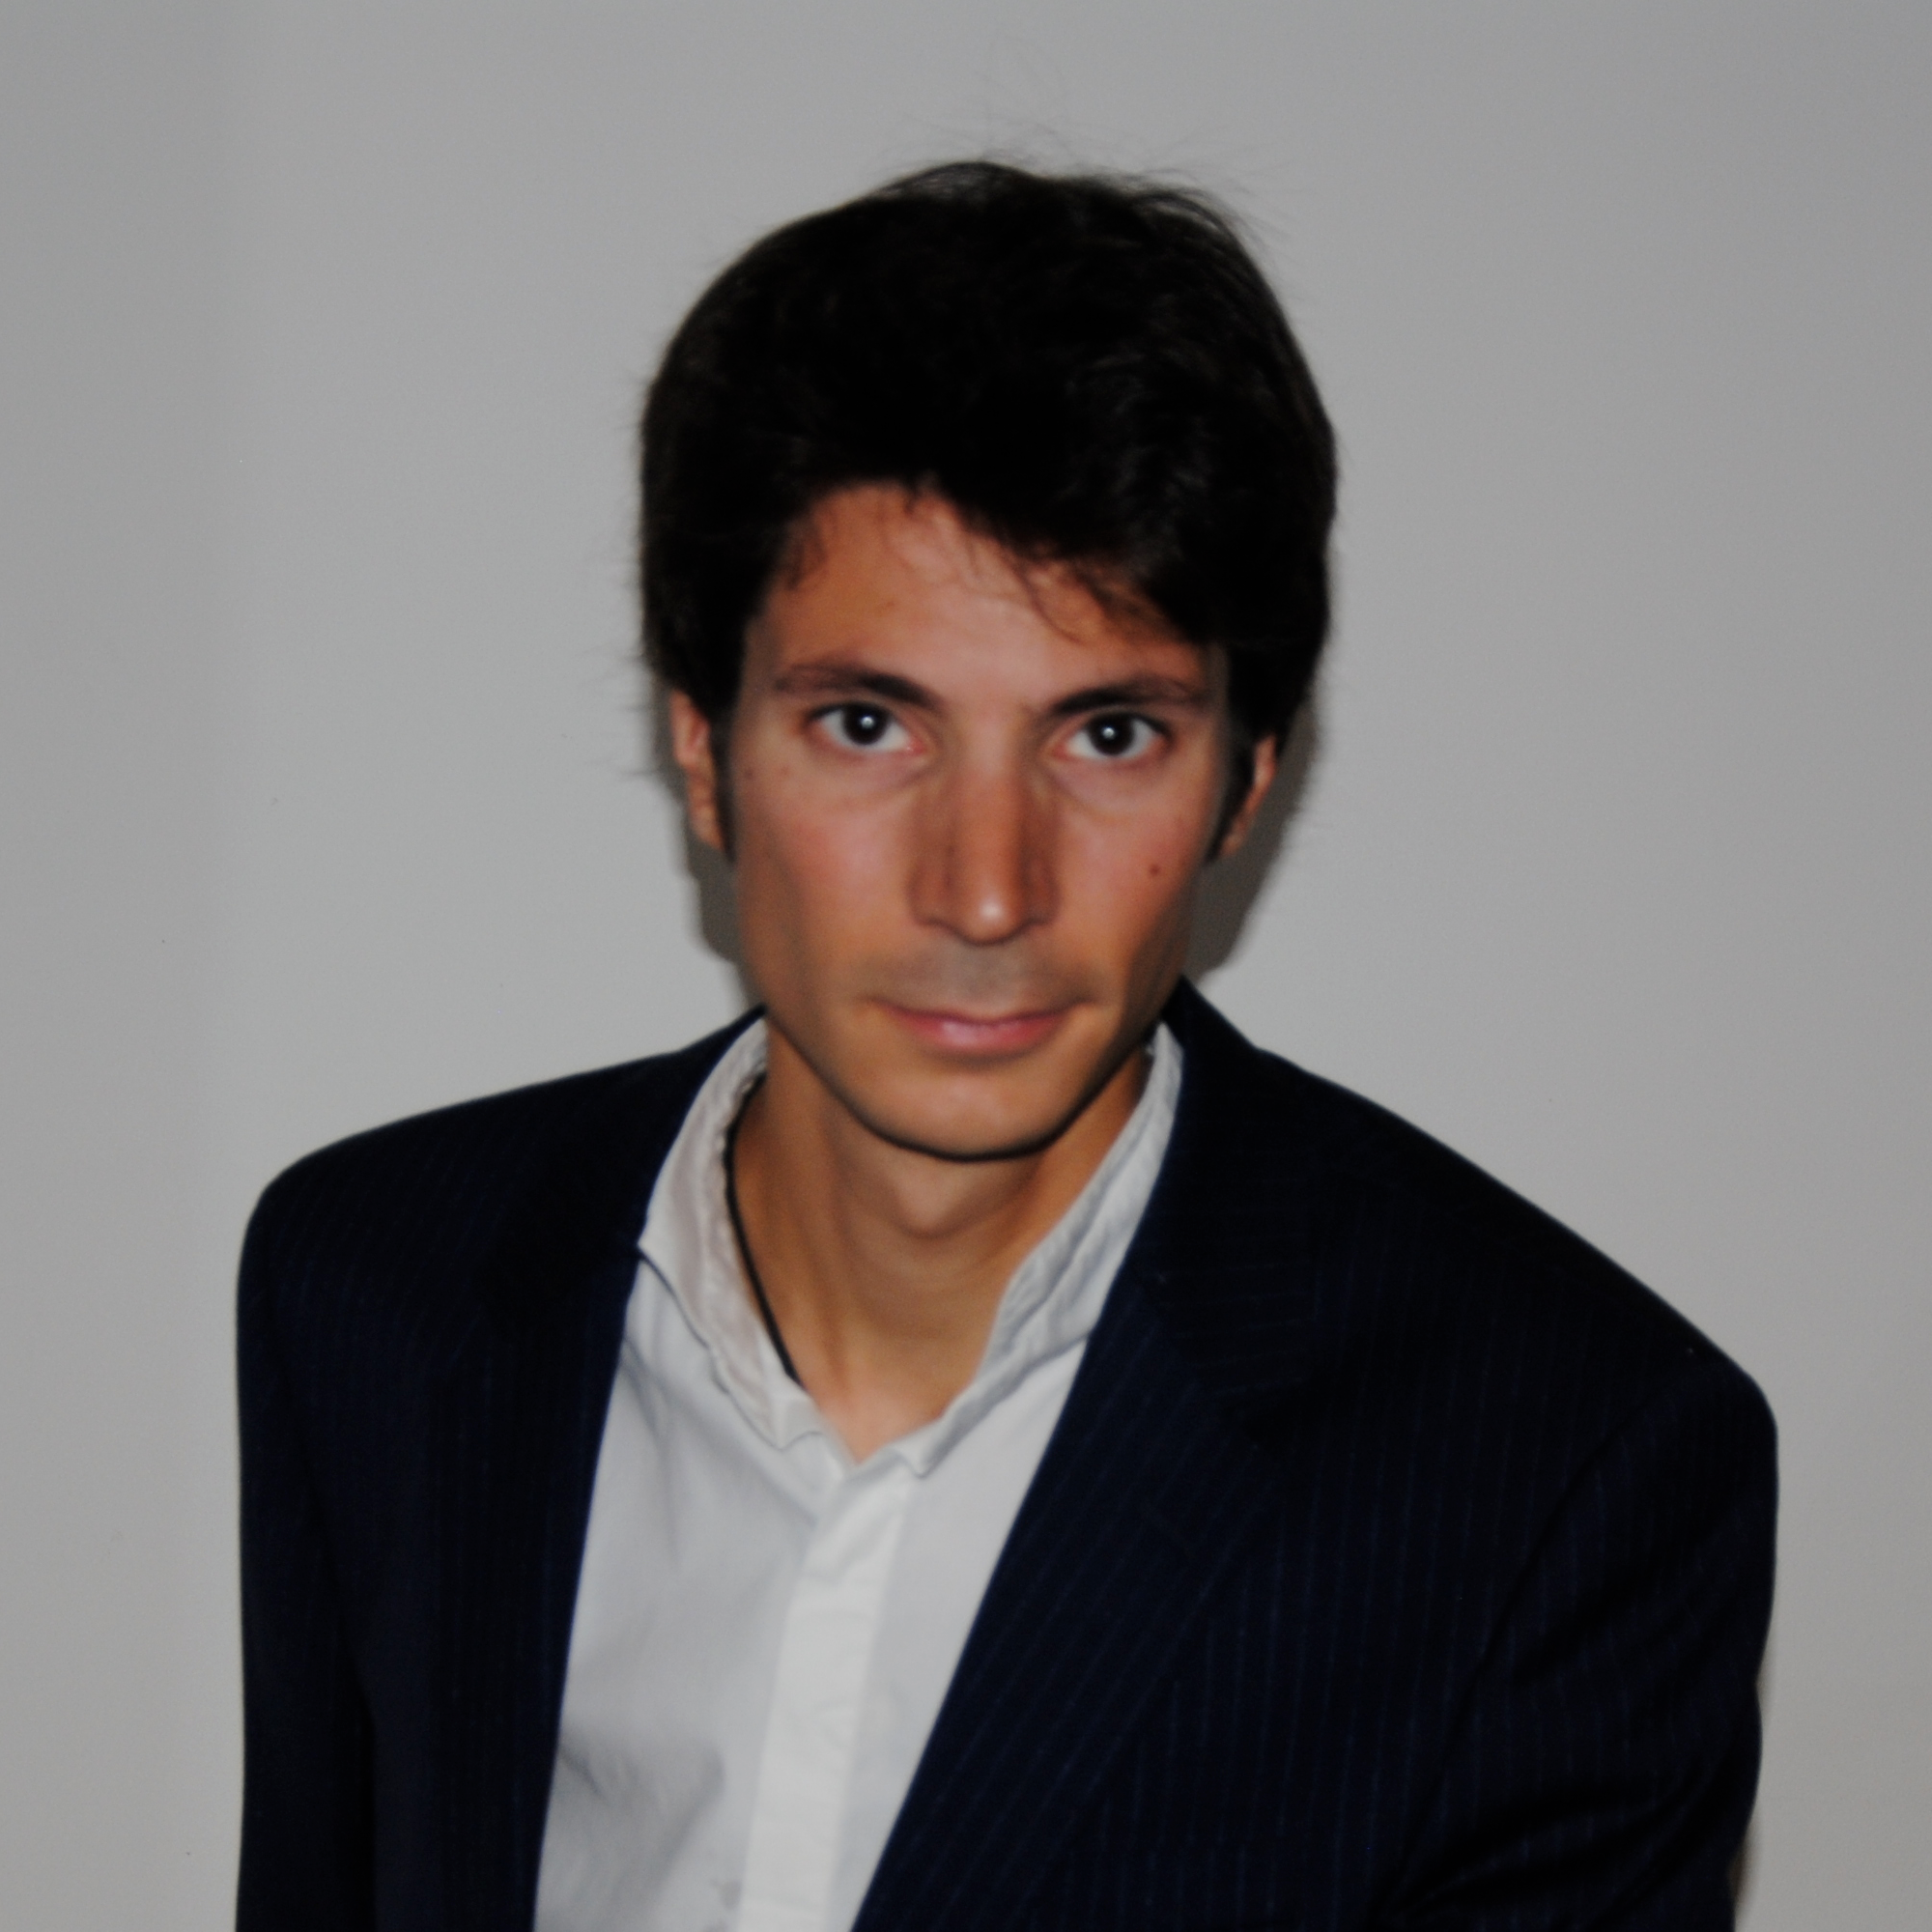
\includegraphics[width=4cm]{images/gauthier}};
                \end{scope}
            \end{tikzpicture}
        \end{flushright}
    \end{figure}

%---------------------------------------------------------------------------------------
%	META SECTION
%----------------------------------------------------------------------------------------

    \vspace{-114pt}

    \metasection{Status}{Fullstack Web Engineer, DevOps Enjoyer}
    \metasection{Fields}{Software Development, System Design, Sports business}
    \metasection{Tech}{TypeScript, React, Node.js, Kotlin, Python, Docker, Git}
    \metasection{Loves}{Trail Running, Ski mountaineering, Chess, Software Craftsmanship}

    \vspace{6pt}

%============================================================================%
%
%	CV SECTIONS AND EVENTS (MAIN CONTENT)
%
%============================================================================%

%---------------------------------------------------------------------------------------
%	EXPERIENCE
%----------------------------------------------------------------------------------------
    \cvsection{\faUserTie}{Experience}

    \cvevent
        {2020 - 2022}
        {Fullstack Web Engineer}
        {UTMB Group, Chamonix \cvflag{FR}}
        {Design software architecture and leading development}
        {Delivered \cvlink{https://utmb.world}{UTMB World} and \cvlink{https://live.utmb.world/utmb/runners/1}{UTMB Live} platforms (React, Next.JS, Nest.JS, Strapi, GraphQL, Meilisearch, Keycloak, MySQL, Redis, d3, Leaflet, Docker, Gatling)}

    \cvevent
        {2018 - 2022}
        {Software Engineer}
        {LiveTrail, Chamonix \cvflag{FR}}
        {Enhance and maintain \cvlink{https://saintelyon.livetrail.net}{LiveTrail} legacy codebase}
        {Reengineered software core (Java, Spring, Maven, React, Redux, Socket.IO) and extended with micro-services (Quarkus, Kotlin, Gradle)}

    \cvevent
        {2015 - 2018}
        {Software Engineer}
        {Atos, Grenoble \cvflag{FR}}
        {Build a sync/async Events Bus for Pôle-Emploi with the SLDBUS Scrum team}
        {Deployed CI/CD and delivered major release (JavaEE, EJB/JMS, Jenkins, Cassandra DB, Oracle DB)}

    \cvevent
        {2013 - 2015}
        {Software Engineer}
        {Bull, Grenoble \cvflag{FR}}
        {Extends software forge with the NovaForge R\&D Team}
        {Integrated GitLab, Jira and created dashboard widgets (J2EE, OSGi/iPOJO, Camel, Vaadin, Apache Karaf, JonAs, Maven)}

    \cvevent
        {2011 - 2012}
        {Technical Lead}
        {Sodifrance, Antananarivo \cvflag{MG}}
        {Lead developers squad in an offshore web agency}
        {Delivered institutional/e-commerce Drupal websites (PHP, HTML, JavaScript, MySQL)}

    %--------------------------------------------------------------------------------------
    %	EDUCATION SECTION
    %--------------------------------------------------------------------------------------

    \cvsection{\faUserGraduate}{Education}

    \cvevent
        {2010}
        {Intern}
        {E-nova Tech, New Delhi \cvflag{IN}}
        {Manage project in an offshore web agency}
        {Delivered institutional Drupal websites}

    \cvevent
        {2005-2010}
        {Master Studies}
        {Université de technologie de Troyes \cvflag{FR}}
        {Classes in computer science : algorithm, database and data-structure}
        {Professionalized in software development and system design}

    \cvevent
        {2009}
        {Semester Abroad}
        {Korean Advanced Institute of Science and Technology \cvflag{KR}}
        {Inter-cultural classes in English, covering special topics in computer science}
        {Developed university projects with Korean teammates}

    %--------------------------------------------------------------------------------------
    %	FOOTER
    %--------------------------------------------------------------------------------------

    \null
    \vspace*{\fill}
    \hspace{-0.25\linewidth}\colorbox{indigo}{\makebox[1.5\linewidth][c]{\mystrut \small
        \textcolor{white}{www.gauthiercart.fr}
        $\cdot$
        \textcolor{white}{github.com/gauthierelcapitan}
        $\cdot$
        \textcolor{white}{https://stackoverflow.com/users/12702817}}}
\end{document}